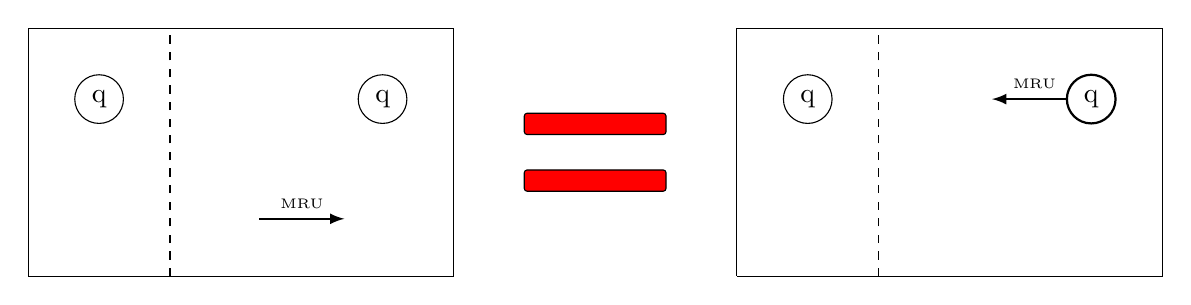
\begin{tikzpicture}[scale=0.9]
  \begin{scope}[shift={(-5,0)}]
    \draw (-1,-.5)--++(6,0)--++(0,3.5)--++(-6,0)--++(0,-3.5);
    \draw[dashed] (-1,-.5)++(2,0)--++(0,3.5);
    \node[circle, draw] at (0,2) {q};
    \eye[black]{.9}{0}{0}{90}
    \node[circle, draw] at (4,2) {q};
    \eye[black]{.9}{2}{0}{90}
    \draw[thick, -latex] (2,0)++(-55*.5+90:0.35)++(0.1,0)--++(.6,0) node[above]{\tiny{MRU}}--++(.6,0);
  \end{scope}

  \begin{scope}[shift={(5,0)}]
    \draw (-1,-.5)--++(6,0)--++(0,3.5)--++(-6,0)--++(0,-3.5);
    \draw[dashed] (-1,-.5)++(2,0)--++(0,3.5);
    \node[circle, draw] at (0,2) {q};
    \eye[black]{.9}{0}{0}{90}
    \eye[black]{.9}{2}{0}{90}
    \draw[thick, -latex] (4,2) node[circle, draw, fill=white] {q} to ++(-.8,0) node[above]{\tiny{MRU}}--++(-.6,0);
  \end{scope}

  \draw[rounded corners=1pt, fill=red] (1,0.7) rectangle ++(2,0.3);
  \draw[rounded corners=1pt, fill=red] (1,1.8) rectangle ++(2,-.3);
\end{tikzpicture}
